\documentclass[a4paper,11pt]{article}

\usepackage[utf8]{inputenc}
\usepackage[italian]{babel}
\usepackage{graphicx}
\graphicspath{ {images/} }

\usepackage{geometry}
 \geometry{
 a4paper
 }
\usepackage[labelfont={bf},textfont=bf]{caption}
% settings

\linespread{1.1}
 \renewcommand{\labelitemi}{$\textendash$}

 \setlength{\parindent}{0ex}

\begin{document}

\author{Giulia Cantini}
\title{A Tandem Queueing Model for Delay Analysis in Disconnected Ad Hoc Networks\\
\vspace{0.5cm}
\Large{An OMNeT++ simulation}}
\maketitle
\date

\tableofcontents

\section{Introduzione}
I tradizionali protocolli di routing \textit{store-and-forward}, che richiedono l'esistenza di un cammino
end-to-end che colleghi sorgente e destinazione, non possono essere utilizzati in reti
soggette a disconnessioni frequenti. Una soluzione che può risolvere questo problema è
sfruttare il movimento dei nodi della rete ed utilizzare il paradigma \textit{store-carry-and-forward}.

In tali reti, chiamate \textit{Delay Tolerant Networks} (DTN), il ritardo di trasmissione dei dati tra i nodi
può risultare elevato a causa delle disconnessioni.

Un importante fattore che caratterizza le DTN è l'opportunità di contatto tra coppie di nodi.
Due nodi sono in contatto se si trovano entro il range di trasmissione l'uno dell'altro,
ovvero ad una distanza tale da consentire lo scambio di pacchetti.

Il modello sviluppato consiste di una rete opportunistica formata da un insieme di tre code
che collaborano tra loro per realizzare il meccanismo opportunistico.

Esso si basa sulle seguenti assunzioni:

\begin{enumerate}
  \item I contatti sono puramente opportunistici, ovvero non si ha nessuna conoscenza
  di quando questi avverranno (protocollo \textit{no-context});
  \item la distribuzione dei tempi di inter-contatto ha media e varianza finite;
  \item il nodo sorgente ha in arrivo un flusso di pacchetti;
  \item i nodi sorgente e destinazione sono fissi, mentre i nodi intermedi sono mobili e
  fungono da \textit{relay};
  \item il modello è basato su due code che sono servite in alternanza da un singolo server.
  Il server è autonomo e non c'è modo di controllarne il movimento;
  \item il nodo mobile salva i pacchetti che provengono dalla sorgente e li inoltra a destinazione;
  \item il nodo mobile non è mai nel \textit{range} di sorgente e destinazione allo stesso tempo.

\end{enumerate}

\section{Modello}

Il modello considerato consiste di 3 sistemi a server singolo first-in-first-out (FIFO) con coda a capacità illimitata, \textit{Q\textsubscript{i}}, i = 1,2,3 in cui i pacchetti arrivano in \textit{Q\textsubscript{1}} e successivamente richiedono il servizio in \textit{Q\textsubscript{2}} prima di raggiungere la destinazione in \textit{Q\textsubscript{3}}. 
Particolare caratteristica del modello è che \textit{Q\textsubscript{2}} si alterna tra le posizioni \textit{L\textsubscript{1}} e \textit{L\textsubscript{2}} in modo che il server di \textit{Q\textsubscript{1}} è disponibile solamente quando \textit{Q\textsubscript{2}} si trova in \textit{L\textsubscript{1}} e il server di \textit{Q\textsubscript{2}} è disponibile solo quando \textit{Q\textsubscript{2}} si trova in \textit{L\textsubscript{2}}. \newline
Inoltre esiste un tempo di \textit{switch-over} da \textit{L\textsubscript{i}} a \textit{L\textsubscript{j}} $(\textit{i} \neq \textit{j},  \textit{j} \in \{1,2\})$
in cui né il server in \textit{Q\textsubscript{1}} né il server in \textit{Q\textsubscript{2}} sono disponibili.\newline
\textit{Q\textsubscript{3}} funge da \textit{sink} e non viene considerata nell'analisi. \newline
\textit{Q\textsubscript{2}} si muove in maniera autonoma, rimanendo in una determinata locazione L per un intervallo di tempo generato da una distribuzione esponenziale (\textit{tempo di permanenza}).\newline
Durante il periodo di disponibilità di un server in \textit{Q\textsubscript{1}} o \textit{Q\textsubscript{2}}, questo può alternare momenti di servizio e momenti in cui è \textit{idle}, in base alla presenza di clienti/pacchetti da servire.

\begin{figure}[h!]
    \centering
    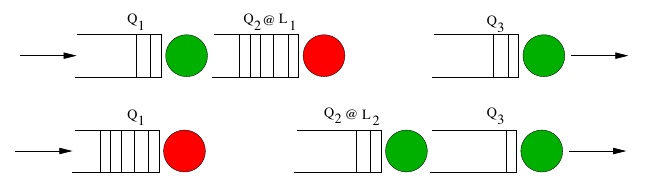
\includegraphics[width=\linewidth]{images/oppnet-model.png}
    \caption{Modello a tre code con una coda mobile.
    Top: Quando \textit{Q\textsubscript{2}} è in \textit{L\textsubscript{1}}, il suo server è down.
    Bottom: Quando \textit{Q\textsubscript{2}} è in \textit{L\textsubscript{2}}, il suo server è up.}
    \label{fig:1}
\end{figure}
\newpage
\section{Implementazione}

Nella rete modellata, denominata \textit{OppNet}, \textit{Q\textsubscript{1}} e \textit{Q\textsubscript{2}} sono due moduli \textit{OppPassiveQueue} serviti da un unico server \textit{S}, \textit{Q\textsubscript{3}} è una coda con server built-in, e sono presenti inoltre una \textit{source} che genera i pacchetti e un \textit{sink} che li raccoglie dopo che hanno attraversato l'intero sistema.\newline

\begin{figure}[h!]
    \centering
    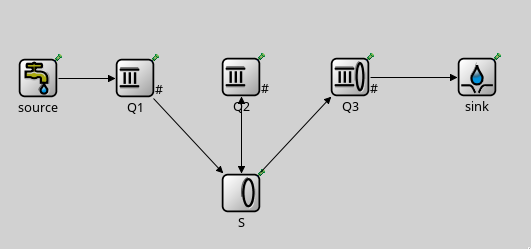
\includegraphics[width=\linewidth]{images/oppnet-mymodel.png}
    \caption{Visualizzazione del file oppnet.ned}
    \label{fig:2}
\end{figure}

Il comportamento di \textit{S} è determinato dalla classe OppServer.cc che estende dalla classe \textit{Server} presente nella libreria \textit{queueinglib}.\newline
Il meccanismo opportunistico è implementato introducendo due nuovi tipi di eventi: \textit{startSwitchEvent} e \textit{endSwitchOverTimeEvent}, che delimitano il periodo di \textit{switch over}, in cui il server non è disponibile per nessuna delle due code: il primo si verifica per segnalare l'inizio dello \textit{switch} ed il secondo per segnalarne la fine.\newline
La non disponibilità del server è espressa dalla variabile booleana \textit{serverIsAvailable}.\newline
Un'altra \textit{flag} \textit{isServingQ1} viene invece utilizzata per controllare quale coda tra \textit{Q\textsubscript{1}} e \textit{Q\textsubscript{2}} deve essere servita.

\begin{figure}[h!]
    \centering
    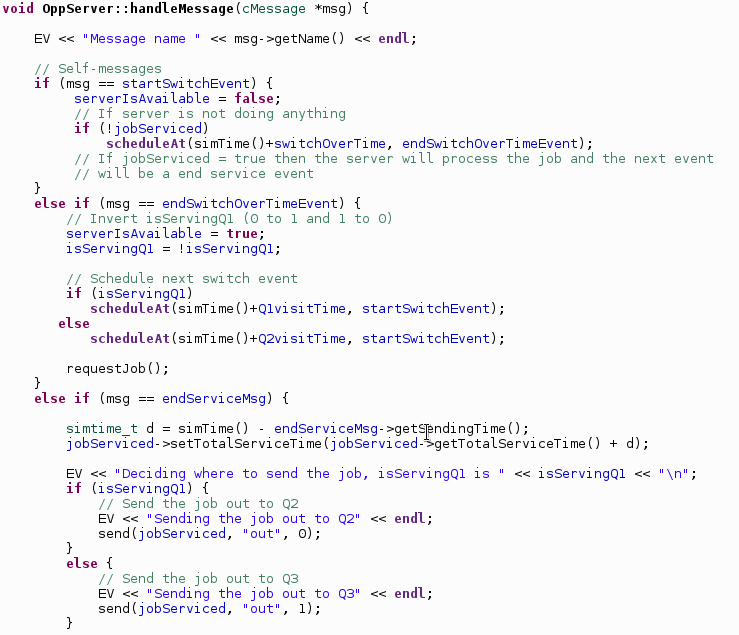
\includegraphics[width=\linewidth]{images/handle-message-oppserver.png}
    \caption{Gestione dello \textit{switch over} e alternanza del server tra le due code \textit{Q\textit{1}} e \textit{Q\textsubscript{2}}.}
    \label{fig:1}
\end{figure}

\section{Simulazione}

% eseguire la simulazione da riga di comando
% ./oppnet-sim -m -n .:../../Scaricati/omnetpp-5.4/samples/queueinglib -l ../../Scaricati/omnetpp-5.4/samples/queueinglib/queueinglib omnetpp.ini -c PreliminarySimulation


\subsection{Transiente iniziale}
\subsection{Risultati}

\section{Conclusioni}

\begin{thebibliography}{90}

\bibitem{K} A. Al-Hanbali, R. de Haan, R. J. Boucherie, J. van Ommeren, \textit{A Tandem Queueing Model for Delay Analysis in Disconnected Ad Hoc Networks.}
\bibitem{K} \textit{OMNeT++ Documentation}, https://docs.omnetpp.org/.
\bibitem{K} \textit{OMNeT++ User Guide}, https://doc.omnetpp.org/omnetpp/UserGuide.pdf.
\bibitem{K} \textit{OMNeT++ Simulation Manual}, https://doc.omnetpp.org/omnetpp/manual/.
\bibitem{K} Emmanuel Paradis, \textit{R for Beginners}, https://cran.r-project.org/doc/contrib/Paradis-rdebuts\_en.pdf.
\end{thebibliography}

\end{document}

%#Misure di prestazioni: 
%#-tempo medio di risposta del sistema (= tempo di soggiorno di un utente nel sistema, dall'arrivo alla partenza) 
%# raccolgo id a src e a dst e conto intervallo di tempo. vedi totalQueueingTime
%# e totalServiceTime in Sink (oppure lifetime) devo contare solo le code? o la generazione del 
%#-numero medio di utenti in coda (ad ogni coda separatamente? entrambe? faccio in code separate perché una somma di utenti non mi sembra molto significativa) vedi queueLengthSignal
%#-throughput di sistema (= media di utenti serviti sull'intervallo di tempo) (n utenti nel sink ad istante t2 - n utenti nel sink ad istante t1)/(t2-t1) 
%# USE LITTLE'S LAW? throughput = n medio di utenti nel sistema (somma di utenti nelle 3 code ) / tempo medio di risposta del sistema